\documentclass{article} % For LaTeX2e
\usepackage{../../tex-style/nips_2014,times}
\usepackage{hyperref}
\usepackage{url}
\usepackage{graphicx}
\usepackage{CJKutf8}
\hypersetup{unicode}
\AtBeginShipoutFirst{\input{zhwinfonts.tex}}
\usepackage{algorithm}  
\usepackage{algorithmic}
\usepackage{amsmath}
\title{Neural Turing Machines}

\author{
 \url{https://www.dosrc.com/}
}


\nipsfinalcopy % Uncomment for camera-ready version

\begin{document}
\begin{CJK*}{UTF8}{gkai}

\maketitle

\section{相关知识}


\textbf{图灵机}:图灵机是一个理论的计算模型,由计算机技术先驱Turing在1936年提出
\begin{center}
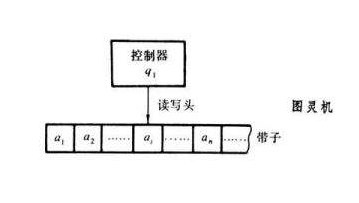
\includegraphics[width=4in]{turing-machines.png}
\end{center}
\textbf{冯·诺伊曼体系结构}:
\begin{center}
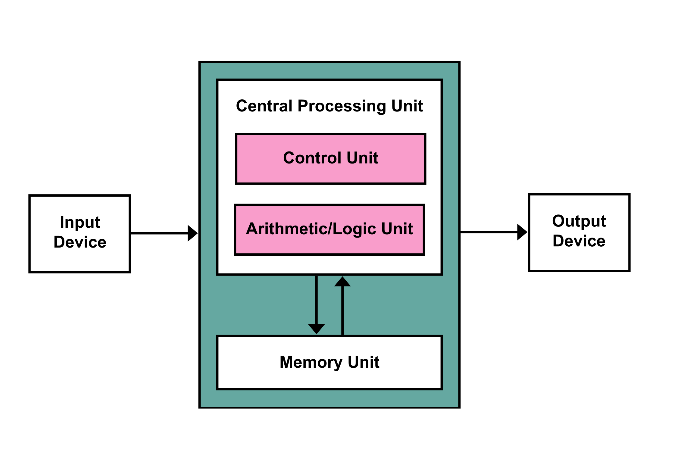
\includegraphics[width=4in]{von-neuman-architecture.png}
\end{center}

\section{神经网络图灵机}
计算机程序在执行计算任务的过程中(Von Neumann, 1945)使用了三个基本机制:初等运算(如算术操作),逻辑控制流(分支循环)和可读写的存储器。虽然现代机器学习理论在建模复杂数据方面取得了广泛的成功,却普遍忽略了对控制流和存储器的使用。本文通过引入外部存储器(external memory)来增强神经网络的能力,神经网络和外部存储器之间通过注意力机制进行交互。新系统可以与图灵机或者冯·诺依曼体系相类比,但每个组成部分都是可微的,可以使用梯度下降进行高效训练。初步的结果显示神经网络图灵机能够从输入和输出样本中推理出简单的算法,如复制、排序和关联性回忆。

\subsection{网络结构}
\begin{center}
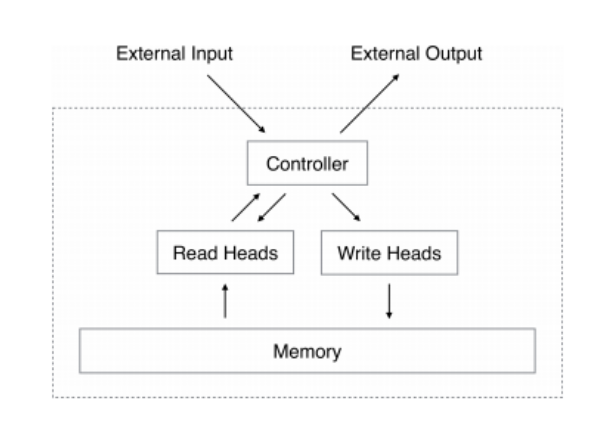
\includegraphics[width=4in]{neural-turing-machines.png}
\end{center}

\subsection{存储器结构}
存储器是一个N行M列的矩阵

\subsection{读存储器操作}
$$ \sum _{i} w _{t}\left( i \right) = 1,\qquad 0 \leq w _{t}\left( i \right) \leq 1,\ \forall i.$$
$$ r _{t} \leftarrow \sum _{i} w _{t}\left( i \right) M _{t}\left( i \right)$$
其中$ \textbf{w} _{t} $是一个N维向量,代表读权重

\subsection{写存储器操作}
$$ \tilde{\textbf{M}} _{t} \left( i \right) \leftarrow \textbf{M} _{t-1} \left( i \right) \left [\textbf{1}- w _{t}\left( i \right)\textbf{e} _{t} \right ] $$
$$ \textbf{M} _{t} \left( i \right) \leftarrow \tilde{\textbf{M}} _{t} \left( i \right) + w _{t}\left( i \right)\textbf{a} _{t} $$

其中$ \textbf{w} _{t} $是一个N维向量,代表写权重

其中$ \textbf{e} _{t} $是一个M维向量,代表擦除权重

其中$ \textbf{a} _{t} $是一个M维向量,代表写入的值向量

\subsection{寻址方式}
\subsubsection{内容寻址}
即按内容的相关性来寻址,读写头先产生一个$\textbf{k} _{t}$的键值,通过与每个内存中的值$\textbf{M} _{t}\left( i \right)$相比较,来产生一个N维的相似度向量$ \textbf{w} ^{c}_{t}$,其表达式如下:
$$ w ^{c}_{t} \left( i \right) \leftarrow \frac{{\rm exp} \left ( \beta _{t}K \left [ \textbf{k} _{t}, \textbf{M} _{t} \left ( i \right ) \right ] \right )}{\sum _{j} {\rm exp} \left ( \beta _{t}K \left [ \textbf{k} _{t}, \textbf{M} _{t} \left ( j \right ) \right ] \right )}$$
在本文中相似度函数$K \left [ \cdot, \cdot \right ]$由余弦相似度给出,如下:
$$ K \left [ \textbf{u}, \textbf{v}  \right ] = \frac{\textbf{u} \cdot \textbf{v}}{\left \| \textbf{u} \right \| \cdot \left \| \textbf{v} \right \|}$$
其中$\beta _{t}$表示注意力集中的精度
\subsubsection{位置寻址}
\paragraph{1.}插值
$$ \textbf{w} ^{g}_{t} \leftarrow g _{t} \textbf{w} ^{c}_{t} + \left ( 1 - g _{t} \right ) \textbf{w} _{t-1} $$
其中${g}_{t}$表示插值的一个门,可理解为一个控制遗忘程度的权重。$w ^{c}_{t}$是由内容寻址产生的权重值,$w _{t-1}$是前一时刻的寻址权重值。
\paragraph{2.}循环卷积
$$ \tilde{w} _{t} \left( i \right) \leftarrow  \sum ^{N-1}_{j=0} w ^{g}_{t} \left( j \right) s _{t} \left( i-j \right)$$
其中$s _{t}$代表循环卷积的向量。循环卷积是为了移动读写头的位置。
\paragraph{2.}锐化
$$ w _{t} \left( i \right) \leftarrow \frac{\tilde{w} _{t} \left( j \right) ^{\gamma _{t}}}{\sum _{j} \tilde{w} _{t} \left( j \right) ^{\gamma _{t}}} $$
其中标量$\gamma _{t}$代表锐化的程度,并且$\gamma _{t} \geq 1$。锐化是防止循环卷积后权重值的分散。

\subsubsection{寻址流程图}
\begin{center}
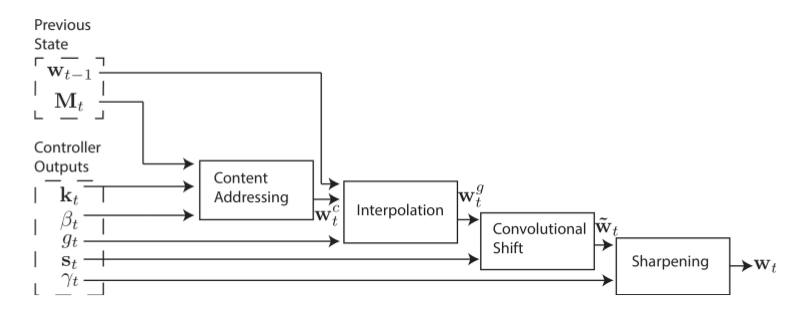
\includegraphics[width=6in]{flow-diagram-of-the-addressing-mechanism.png}
\end{center}

\section{实验}
\subsection{复制任务}
复制任务的学习训练曲线:
\begin{center}
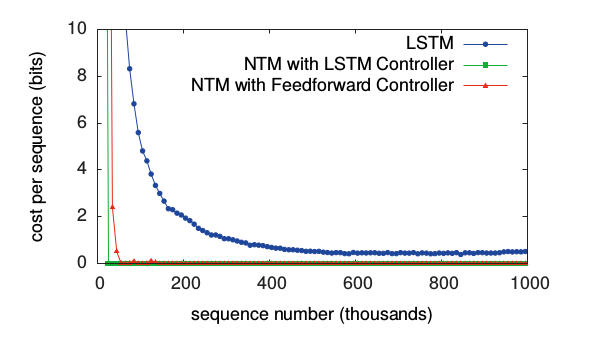
\includegraphics[width=4in]{copy-learning-curves.png}
\end{center}

NMT在复制任务上的泛化能力:
\begin{center}
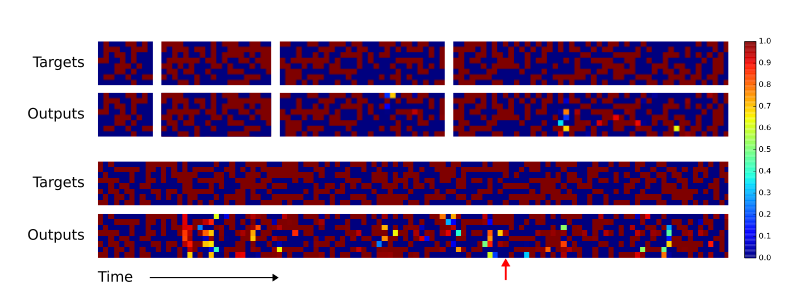
\includegraphics[width=4in]{nmt-generalisation-on-the-copy-task.png}
\end{center}

LSTM在复制任务上的泛化能力:
\begin{center}
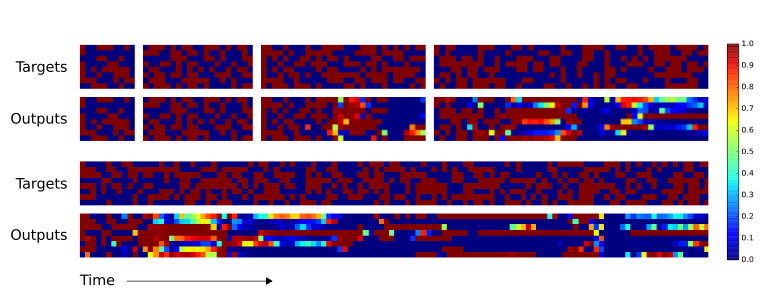
\includegraphics[width=4in]{lstm-generalisation-on-the-copy-task.png}
\end{center}

NMT在复制任务上的存储器使用情况:
\begin{center}
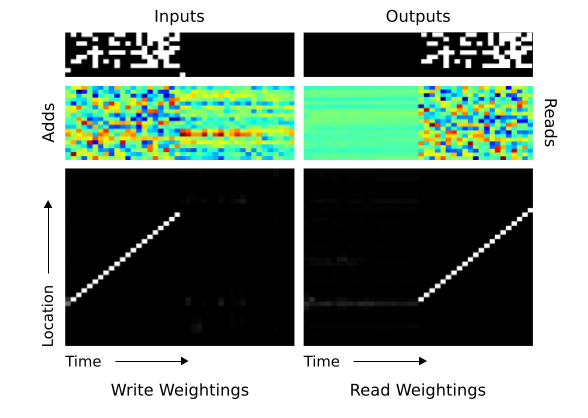
\includegraphics[width=4in]{nmt-memory-use-during-the-copy-task.png}
\end{center}
可以看出基本和低级语言编写的程序存储器使用情况一致。
\subsection{重复复制任务}
重复复制任务的学习训练曲线:
\begin{center}
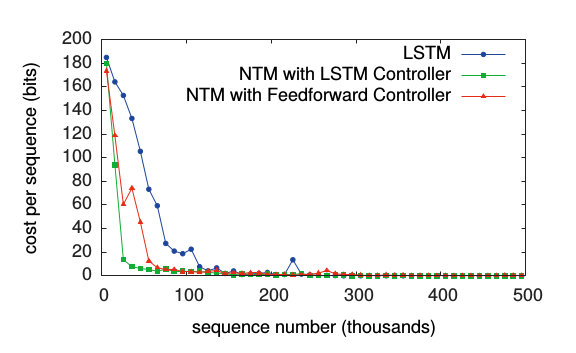
\includegraphics[width=4in]{repeat-copy-learning-curves.png}
\end{center}

NMT在重复复制任务上的泛化能力:
\begin{center}
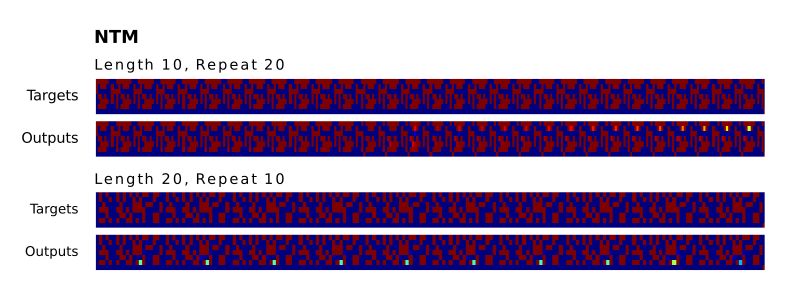
\includegraphics[width=4in]{nmt-generalisation-on-the-repeat-copy-task.png}
\end{center}

LSTM在重复复制任务上的泛化能力:
\begin{center}
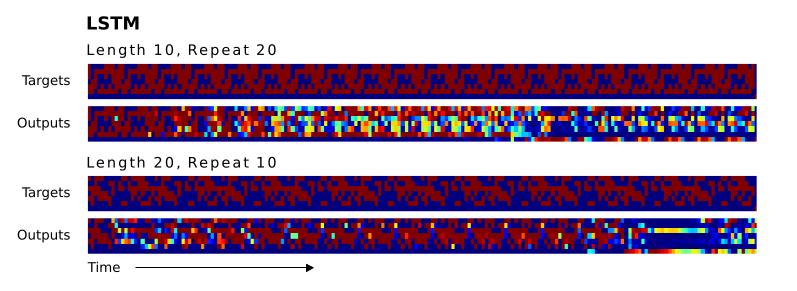
\includegraphics[width=4in]{lstm-generalisation-on-the-repeat-copy-task.png}
\end{center}

NMT在重复复制任务上的存储器使用情况:
\begin{center}
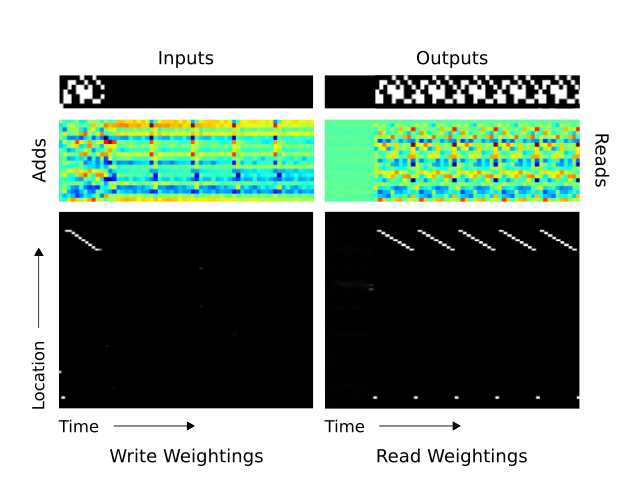
\includegraphics[width=4in]{nmt-memory-use-during-the-repeat-copy-task.png}
\end{center}
可以看出基本和低级语言编写的程序存储器使用情况一致。

\end{CJK*}
\end{document}